
%%%%%%%%%%%%%%%%%%%%%%%%%%%%%%%%%%%%%%%%%%%%%%%%%%%%%%%%%%%%%%%%%%%%%%%%%%%%%%%%

%        1         2         3         4         5         6         7         8

\documentclass[letterpaper, 10 pt, conference]{ieeeconf}  % Comment this line out if you need a4paper

%\documentclass[a4paper, 10pt, conference]{ieeeconf}      % Use this line for a4 paper

\IEEEoverridecommandlockouts                              % This command is only needed if 
                                                          % you want to use the \thanks command

\overrideIEEEmargins                                      % Needed to meet printer requirements.


\usepackage{graphics} % for pdf, bitmapped graphics files
\usepackage{epsfig} % for postscript graphics files
\usepackage{mathptmx} % assumes new font selection scheme installed
\usepackage{times} % assumes new font selection scheme installed
\usepackage{amsmath} % assumes amsmath package installed
\usepackage{amssymb}  % assumes amsmath package installed

\usepackage[font=small,labelfont=bf]{caption}

% Other package
\usepackage{tikz}
\usepackage{graphicx}
\usepackage{caption} 
\usepackage{subcaption}
\usepackage{multirow}
\usepackage{array}
\usepackage{booktabs}
\usepackage{hyperref}

\usepackage{pdfpages}
\usepackage{caption}
%\usepackage{geometry}
\usepackage{import}
\usepackage{standalone}

\title{\LARGE \bf
  Team-JSK: MBZIRC Progress Report
}
\author{Team JSK$^\dagger$% <-this % stops a space
  \\ JSK Lab, Graduate School of Information Science and Technology, The University of Tokyo \\
  7-3-1 Hongo, Bunkyo-ku, Tokyo, Japan 113-8656.  \\
\thanks{$^{*}$ %JSK Lab, Graduate School of Information Science and Technology, The University of Tokyo,  7-3-1 Hongo, Bunkyo-ku, Tokyo 113-8656, Japan.  
{$^\dagger$\tt\small http://www.jsk.t.u-tokyo.ac.jp}
}}
\begin{document}

\maketitle
\thispagestyle{empty}
\pagestyle{empty}


\section{Introduction}
This document provides a report of Team JSK's progress in preparing for the Mohamed Bin Zayed International Robotics Challenge (MBZIRC). The team consists of members from the JSK Laboratory at the University of Tokyo. The JSK Lab, founded in early 1980’s, has a long history of robotics research with focus on areas including humanoids, drones, robotics manipulation, and perception, and the lab has experience in participating in robotics challenges including the DARPA Robotic Challenge and the Amazon Picking Challenge.

\subsection{Project Personnel}
Team JSK is made of eleven members: Prof. Masayuki Inaba, Prof. Kei Okada, Dr. Yohei Kakiuchi, Dr. Wesley Chan, Bakui Chou, Xiangyu Chen, Krishneel Chaudhary, Kohei Kimura, Yuki Furuta, and Hiroto Mizohana. The team is roughly divided into three groups corresponding to each task with groups having overlapping personnel.


%That is a professor, a associate-professor, a lecturer, a researcher, 4 Phd students and 2 Master students. 
%Teachers mainly focus on manage the whole team schedule, design hardware and software architecture, provide advices and give ideas for all the tasks. The rest researcher and students are divided into three groups, 
%one for computer vision development for all the tasks, one for task 2 and one for task 1 and 3.


\section{CHALLENGE 1: LANDING UAV ON A MOVING VEHICLE}


%Copyright (C) 2016 by Krishneel@JSK Lab, The University of Tokyo

\documentclass{standalone}
\begin{document}

\subsection{Hardwares}

is done by Bakui

\end{document}

%Copyright (C) 2016 by Krishneel@JSK Lab, The University of Tokyo

\documentclass{standalone}
\usepackage{footnote}
\usepackage{hyperref}
\usepackage{graphicx}

\begin{document}

\subsection{Software}

The software, including motion planning, visual perception and virtual simulation, are developed on the ROS robot operating system, and we use Gazebo for performing simulations \footnote{\url{https://github.com/start-jsk/jsk_mbzirc}}. We use the Gazebo simulator for testing and planning our strategy and for customizing our hardware and software. The visual perception component carries out target (heliport) localization of the moving vehicle, and we plan the efficient approaching and landing strategy based on the motion of both the UAV and the vehicle. Since we use Nvidia TX1 embedded processor for fast computations on GPU, our algorithms for \textit{task 1} and \textit{task 3} are developed in CUDA-C, C/C++ and Python. 

% \begin{figure}[t]
%   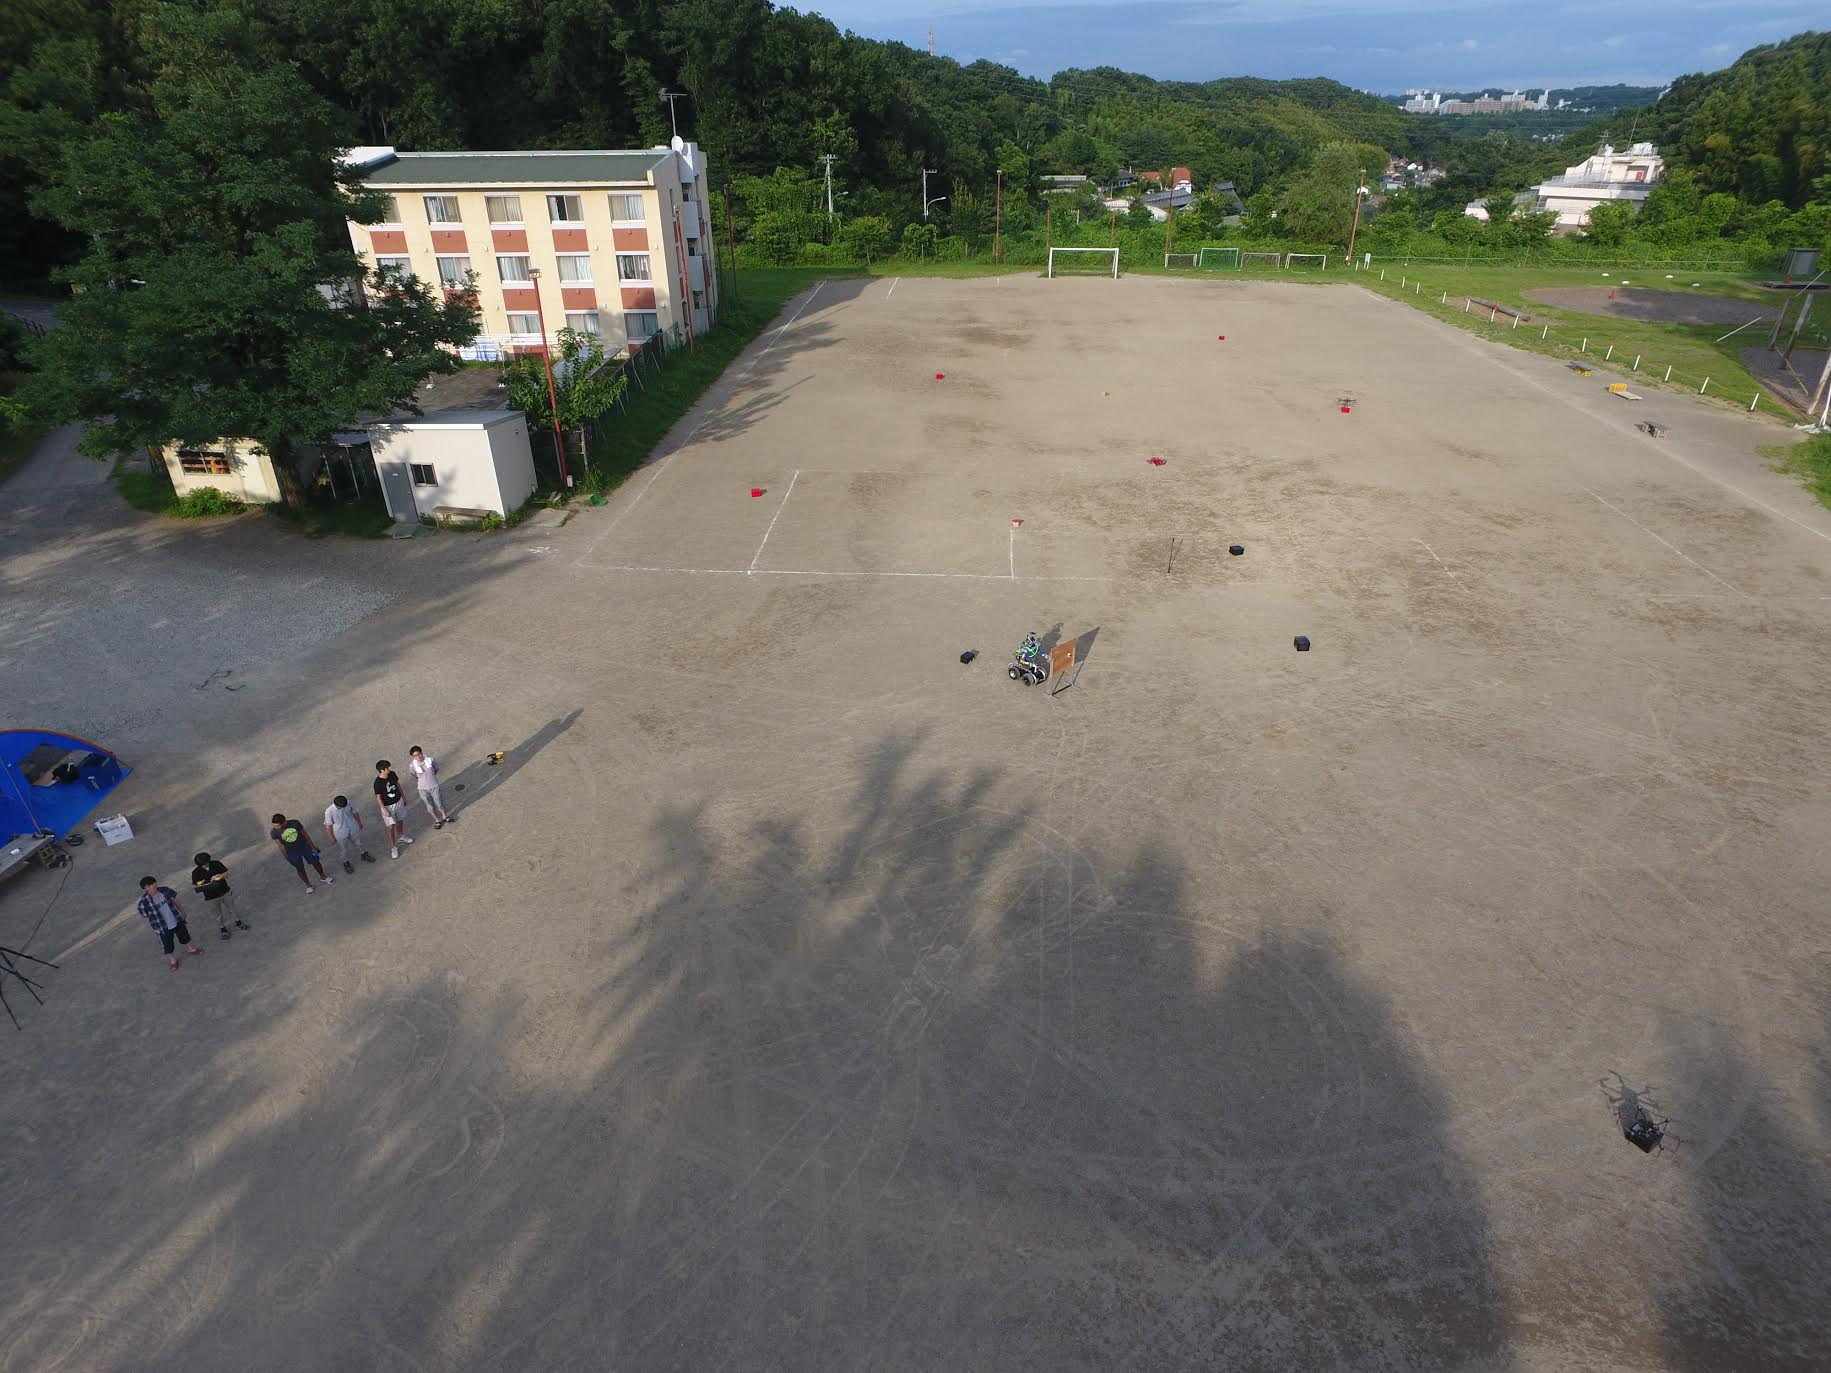
\includegraphics[width=\columnwidth, trim={2cm 5cm 3cm 7cm},clip]{sections/task1/images/testbed}
%   \caption{Testbed for outdoor testing in Hachioji, Tokyo, Japan}
% \end{figure}


\subsection{General Approach}

%\textbf{Vehicle And Heliport Detection}: 
We use the heliport model to train a linear classifier for detection of the landing region. Since heliport model is known, it is used as an a priori for learning. Once the heliport is detected, a visual object tracker running in real time on-board is autonomously initialized to start tracking the target region. We use a robust tracking algorithm with efficient drift compensation algorithm to avoid lost of target when the UAV is in motion. Our visual tracking algorithm is also able to recover the target even if it went completely out of view. Once the target is localized, the UAV uses pose information from the visual tracker to navigate towards the target. 



\subsection{Future Plans}
The future work on software for task 1 involves testing the completed software on the customized UAV which is currently under development. This involves fine tuning the current simulator version of our software. Considering the challenges in outdoor environment such as abrupt changes in image space, winds speeds etc. the landing strategy might vary significantly from the simulator version. One very important aspect of autonomous systems which we like to implement is the ability of the UAV to recover from erroneous decision, false positives that might result in highly cluttered and unstructured scene.

%we will have to improve our current landing strategy in the real world. 

\end{document}

%% insert yout latex module file here. the contents should go to the tasks folder under section

\section{CHALLENGE 2: OPERATING A VALVE STEM}

%Copyright (C) 2016 by Krishneel@JSK Lab, The University of Tokyo

\documentclass{standalone}

\usepackage{hyperref}
\usepackage{footnote}
\usepackage{graphicx}

\begin{document}

\subsection{Hardware}
Our robot consists of an upper body humanoid on a high-power mobile base(Fig.\ref{fig:figure1}). The robot is equipped with a stereo camera, a long range laser sensor, a global positioning system (GPS), and a custom made gripper. The gripper consists of a magnet embedded link actuated by a servo motor as shown in Fig.\ref{fig:figure2}. The wrist is also equipped with a six axis force torque sensor. 


\begin{figure}
  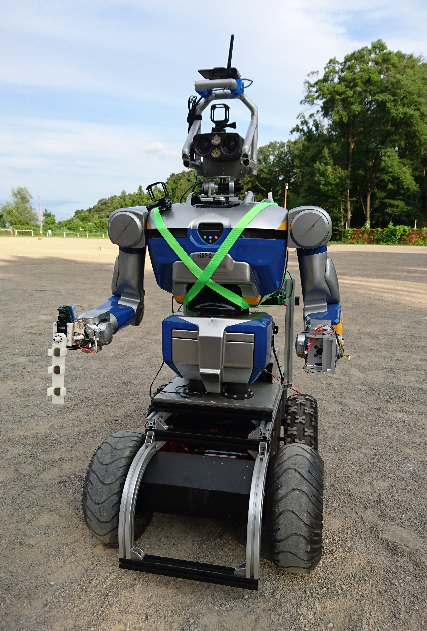
\includegraphics[height=2.5in, width=1.5in]{sections/task2/images/figure1}
  \caption{HRP2 robot platform for task2}
  \label{fig:figure1}
\end{figure}

\subsection{Software}

For task 2, the softwares are also implemented on ROS environment with utilization of multithreading for fast computation. Euslisp programming language from JSK lab was used for kinematics simulation and robot control. OpenCV and in-house developed algorithms
 \footnote{\url{https://github.com/jsk-ros-pkg/jsk_recognition}} are used for recognition and perception.


 \subsection{General Approach}
 \textbf{Navigation}: Our approach is to use the long range laser sensor and the GPS for searching and navigating to the panel when the robot is far from the robot and is out of range for the stereo camera. As the panel becomes closer than the minimum range of the laser sensor, the robot will then switch over to use the stereo camera. Our high-powered mobile base can reach up to 4m/s and can drive through various outdoor terrains. 

\textbf{Wrench and valve stem detection}: We experimented and compared infrared camera with stereo camera, and we have decided to use stereo camera for close range perception, since infrared cameras tend to fail in outdoor sunny environments, and cannot sense objects that are too close to the robot. 

We detect the wrench by using Edge detection, Hough transform and K-means. Firstly, we select a region include 6 wrenches on the camera image(Fig.\ref{fig:figure3}A). We apply hough line transform to the edge image of selected region and extract lines which have large slope, then apply K-means(K is 6) to extracted lines. The size of wrenches can be estimated from classified lines, but the position of wrenches estimated from lines is not correct(Fig.\ref{fig:figure3}B). Therefore we use Hough circle transform to detect the hanger on image(Fig.\ref{fig:figure3}C) and get depth from point cloud(Fig.\ref{fig:figure3}D). Thus, we can detect the size and position of wrenches.  

We also select the region on the camera image to detect the valve stem(Fig.\ref{fig:figure3}A). We estimate the plane from the point cloud in the selected region, extract the points witch exist in front of the plane(Fig.\ref{fig:figure3}E). The centoroid of the extracted points is considered as the position of the valve stem(Fig.\ref{fig:figure3}F).

\textbf{Picking the wrench}: Our robot picks up the wrench by aligning the gripper with the wrench, moving the gripper toward the wrench, and letting the magnets pull the wrench into the gripper. The gripper is designed so that the wrench is grasps firmly, but with some movement possible for passive compliance.

\textbf{Wrench fitting and turning}: To fit the wrench head onto the valve stem, we use force feedback from the wrist to gauge the tool contact state. The robot first moves its gripper above the detected position of the valve stem. Due to error in detection or calibration, the wrench head could be directly above the valve stem or it can be slightly misaligned (Fig.\ref{fig:figure4}A, B). The robot moves its gripper down, until a force in the vertical direction is detected, indicating that the wrench has come in contact with the valve stem. Once it detects contact with the valve stem, the wrench can be in one of the contacts states as shown in Figure 1 The robot then moves its gripper in the horizontal direction in a widening zigzag pattern. Depending on the forces it detects, the robot then begins to turn the wrench, or adjusts its gripper positon and retries to fit the wrench (Fig.\ref{fig:figure4}).

\begin{figure}
  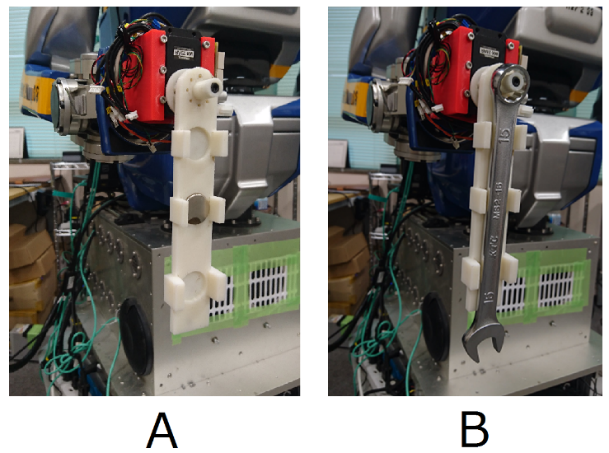
\includegraphics{sections/task2/images/figure2}
  \caption{Custom made magnetic gripper.}
  \label{fig:figure2}
\end{figure}

\begin{figure}
  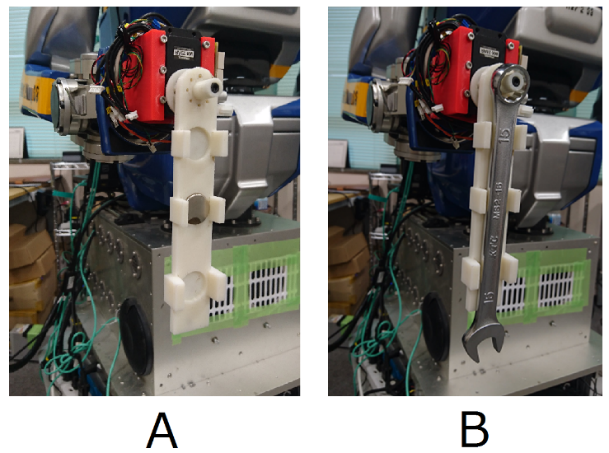
\includegraphics{sections/task2/images/figure3}
  \caption{Wrench and valve stem detection.}
  \label{fig:figure3}
\end{figure}

\begin{figure}
  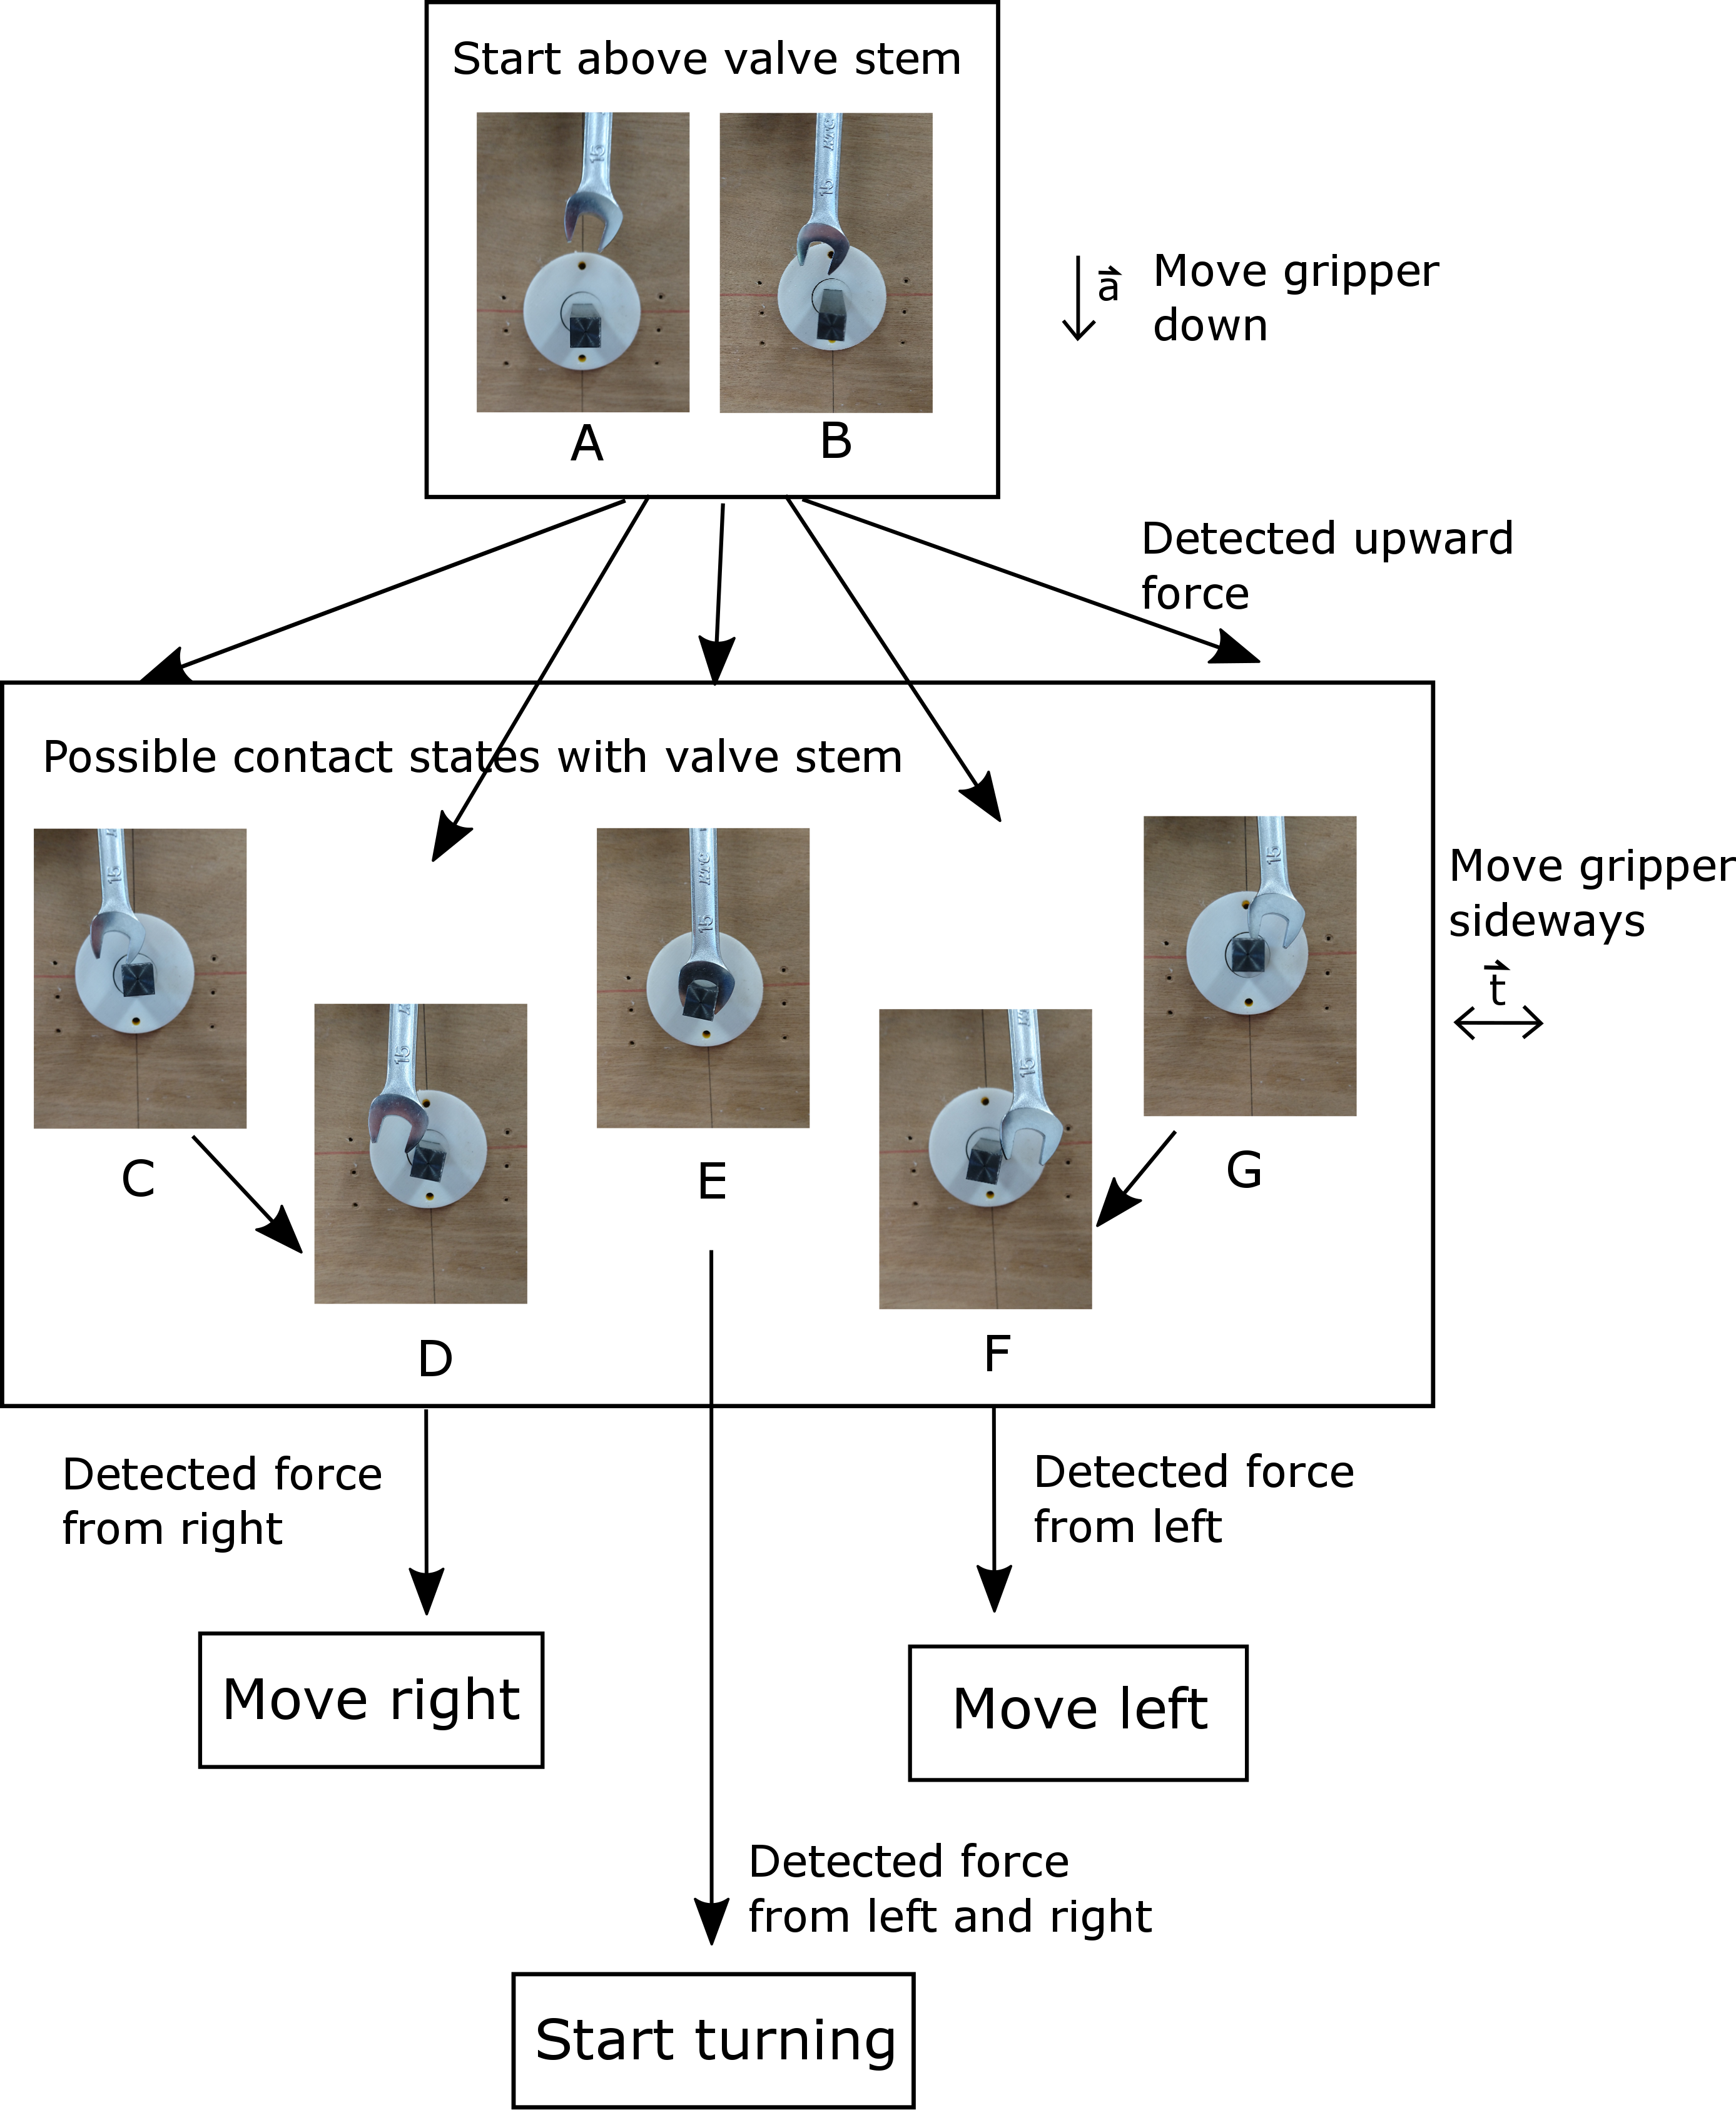
\includegraphics[width=\columnwidth]{sections/task2/images/figure4}
  \caption{Using force fitting for wrench fitting}
  \label{fig:figure4}
\end{figure}


\subsection{Results Achieved to Date}
We have completed the prototypes of our mobile base and customized gripper. The entire robot has been assembled and all sensors are functional. The robot can be operated through teleoperation, and we have been able to successfully complete challenge 2 using full teleoperation indoors and outdoors. 
Recognition of the wrenches and the valve stem has also been implemented. Once we select the region to detect wrenches and valve stem, they will be detected autonomically.
We experimented with wrench fitting and turning with different initial wrench alignments. Among twenty trials, we were able to achieve a 95$\%$ success rate with only one failed trial. 
We have also tested our system for performing the entire challenge 2 with partial autonomy in outdoor experiments. In our experiments, we used teleoperation to drive the robot’s mobile base, allowed the robot to detect the wrenches and valve stem with human supervision, and grasp, fit, and turn the wrench with full autonomy. In our fastest run, we were able to complete challenge 2 in less than ten minutes. This time can be easily shortened as many parts of our code had deliberate pauses for debugging and testing purposes.

\subsection{Future Plans}
Our future plans include speeding up our task completion time, enabling autonomous navigation of the mobile base, autonomous search of the panel, full autonomous wrench and valve stem detection, and failure detection when grasping, fitting, and turning the wrench. We will also consider and compare alternative wrench detection, and wrench fitting methods. Currently, the valve stem we have been operating has very little resistance. While we have successfully turned a valve stem with 5Nm resistance, our gripper prototype broke after turning a quarter turn. We have already strengthened our gripper design, and as future work, we will be testing with valve stems having higher torque resistance.  Finally, we are also considering the potential use of another robot platform that is more lightweight and allows us to more easily transport it from Japan to the competition venue. 

\end{document}


\section{CHALLENGE 3: SEARCH, PICK AND PLACE}



%Copyright (C) 2016 by Krishneel@JSK Lab, The University of Tokyo

\documentclass{standalone}
\begin{document}

\subsection{Hardware}
For task 3, we used two types of UAVs; the $Hawk$ which is similar to the one used in task 1 and a transformable UAV called the $Snake$.
Since all the UAVs uses the same custom built control board, the central control hardware components almost the same as those used for task 1, except that we designed an additional PCB board for controlling the Electronic-Magnet. We equipped 5 Electromagnets on the UAV and build the attachment with tactile sensors. The electromagnet control board is connected to the central control unit through CAN bus.

The $Snake$ has a snake-like structure with for propeller units connected by actuated joints. It is capable of changing its configuration during flight, and allows grasping of objects by enclosing its body around the object. 

\subsection{Software}
As with other tasks the software are build using ROS and some functionalities are shared with task 1. Point Cloud and OpenCV libraries are used for visual perception. % target detection and motion planning are different.

\subsection{General Approach}
%The software system is based on ROS(Robot Operation System). We write our algorithm to the every single node and communicate with each node. 
\subsubsection{Overall Strategy}
We divide the task into three states: Search, Pick, and Place. The UAVs are always in one of these three states and the states automatically transition into the next one if the certain conditions are satisfied as illustrated in Fig. \ref{t3}A. In the "Search" state, the drone will traverse to the center of the arena and randomly generate a search end-point, the treasure detector will run while the drone is searching. Once the object is detected and locked, a pick motion will be generated in the "Pick" state, the UAV will turn on the electromagnet and approach the treasure (for the $Hawk$) or enclose its body around the treasure (for the $Snake$). The state transition is signalled by the trigger of the tactile sensor. Once the electromagnet of the $Hawk$ has caught the treasure or the body of the $Snake$ has enclosed the treasure, the UAV transition into the next state. In the "Place" state, the UAV will fly directly to the placing zone and find the box to place the treasure. After releasing the treasure into the place box, the UAV re-enters the "Search" state and loops until the task is completed.

 \begin{figure}%[hb]
    \begin{center}
      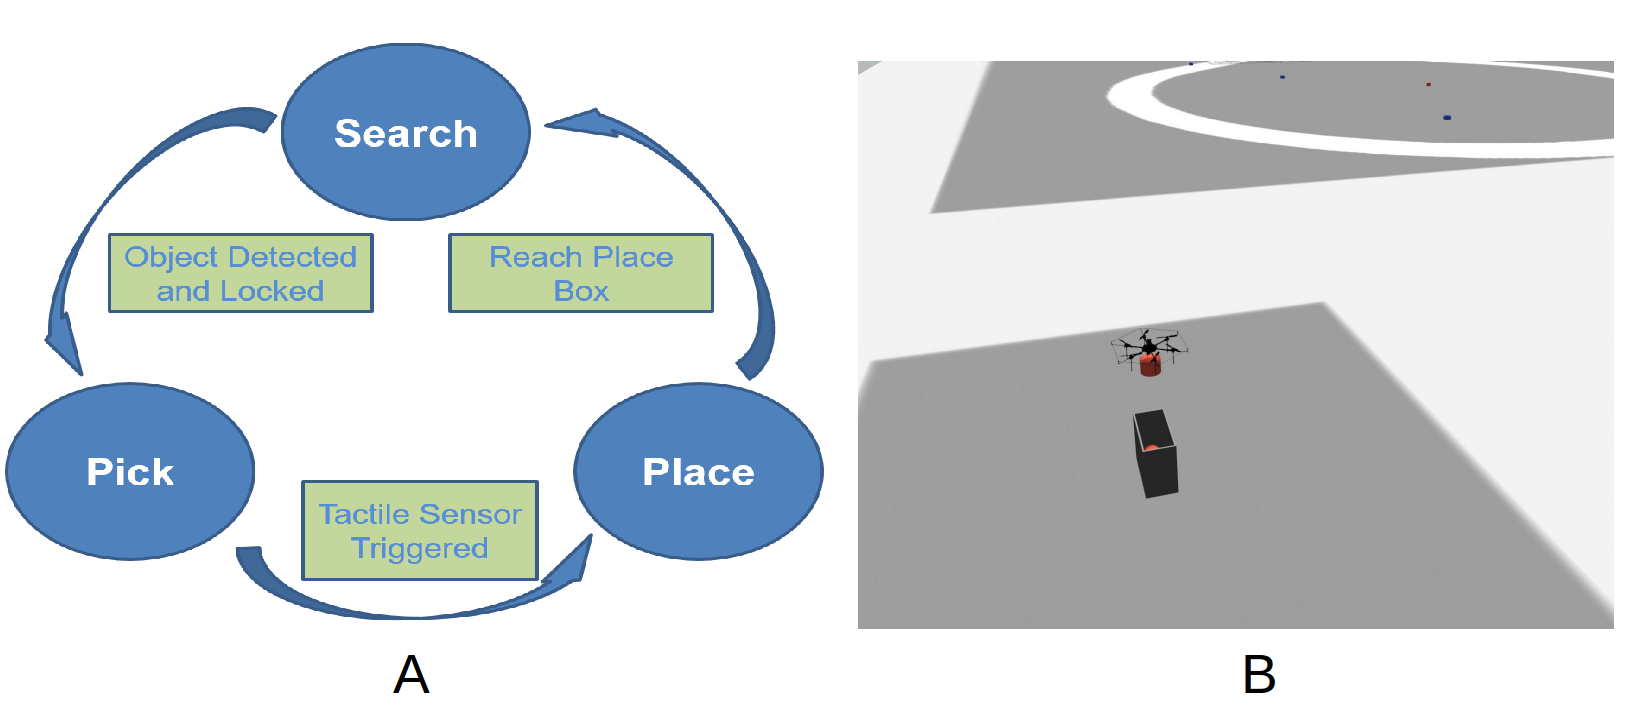
\includegraphics[keepaspectratio=true, width=1\linewidth, height=0.30\textheight]{img//task3.png}
    \end{center}
    \caption{Task 3 Demonstration}
    \label{t3}
  \end{figure}



\subsubsection{Treasure Detection}
As the treasures have distinct color features, we first used a simple detection method to detect the treasures. 
The inputs are 3D points $p_i$ from the Stereo sensor and the RGB image projection onto the ground by the projection matrix computed using the known camera parameters. %We first apply 
HSI color filter is applied to obtain the 3D point candidates of the treasures from the point cloud data. Next we apply Euclidean clustering to the filtered point cloud $P_{hsi}$. Euclidean clustering technique can organize points into clusters with respect to distance features in 3D space. For $\forall p_i, p_j \in P_{hsi}$, clusters $O_i = \{p_i \in P_i\}$ and $O_j = \{p_j \in P_j\}$ are obtained by:
\begin{equation}\label{eq3-1}
min||p_i - p_j|| \geq d_{threhold} 
\end{equation}
After we obtained all the clusters, we apply a simple tracker to every cluster center and as we continue to detect the same cluster over time space, the weight of the tracker is increased to boost the confidence of tracking. For clusters that are not always detected the confidence are slowly decreased and removed from the treasure candidates vector. The UAV will lock on to the cluster candidate when the weight is large enough and switch into the "Pick" mode to approach the treasure.

\subsection{Results Achieved to Date}
We performed full automatic simulation in gazebo environment as shown in Fig.\ref{t3}B. To fully simulate the real scene, we add noise and outliers to the detection. In simulation, the UAV takes almost 70 $seconds$ to detect, pick and place a single object. 
% we believe we can do that better. 
With the real robots, we tested tele-operation control, and both the $Hawk$ and the $Snake$ were able to grasp the treasure and pick and place it into a specified box. 

\subsection{Future Plans}
In our next steps, we will use three UAVs in coordination to complete the task which will not only decrease the time but also can be used to transport larger treasures which a single UAV might not be able to lift. We will also be carrying out more experiments on the real robots to test the detection and motion planning algorithm that have been verified in simulation.


\end{document}


\section{GRAND CHALLENGE}

%Copyright (C) 2016 by Krishneel@JSK Lab, The University of Tokyo

\documentclass{standalone}

\usepackage{graphicx}
\usepackage{float}
\floatstyle{boxed} 
\restylefloat{figure}

\begin{document}


\begin{figure*}[!b]
   \newcommand \ilenght{0.1}
   \newcommand \iheight{2.0in}
   \newcommand \iwidth{0.23\textwidth}
   \centering
   
   \subcaptionbox{
     \scriptsize{}\label{fig3:a}}{\includegraphics[width=\iwidth, height=\iheight]{sections/grand/images/DJI_0028}}\hspace{1.1em}%
   \subcaptionbox{
     \scriptsize{}\label{fig3:b}}{\includegraphics[width=\iwidth, height=\iheight]{sections/grand/images/DJI_0059}}\hspace{1.1em}%
   \subcaptionbox{
     \scriptsize{}\label{fig3:c}}{\includegraphics[width=\iwidth, height=\iheight]{sections/grand/images/DJI_0079}}\hspace{1.1em}%
   \subcaptionbox{
     \scriptsize{}\label{fig3:d}}{\includegraphics[width=\iwidth, height=\iheight]{sections/grand/images/DJI_0092}}\hspace{1.1em}%
   \caption{JSK--Team testbed setup at Hachioji, Tokyo, Japan}
   \label{fig:objects}
 \end{figure*}


\subsection{Setup of TestBed}

We have prepared our testbed where we will perform the outdoor testing in the real world is located in Hachioji, Tokyo, Japan. 

 \subsection{Future Work}
 Once we complete each of the three tasks above, for the grand challenge we will combine each of the 3 tasks above, however we plan to make some changes such as UAV to UAV and UAV to UGV communications such that all the robots are able to collaborate in completing the tasks.
 

\end{document}

%\section{Future Plan}

\end{document}
